%%%%%%%%%%%%%%%%%%%%%%%%%
% Dokumentinformationen %
%%%%%%%%%%%%%%%%%%%%%%%%%
\title{TSM\_EmbHardw}
\author{David Wright}

\documentclass[10pt,twoside,a4paper,fleqn]{scrartcl}

\usepackage{longtable}
\usepackage{hhline}
\usepackage{textcomp}
\usepackage{float}

\include{./header/zusammenfassung}

\usepackage{colortbl}
\definecolor{lightgrey}{rgb}{0.9,0.9,0.9}
\usepackage{tikz}

\newcommand{\avIntSp}[1]{$_{\textcolor{HSRHematite}{\mbox{\small{AvalonIntSpec p. #1}}}}$}
\newcommand{\weekDoran}[1]{$_{\textcolor{HSRBlue}{\mbox{\small{Slides Doran  week #1}}}}$}
\newcommand{\weekPageDoran}[2]{$_{\textcolor{HSRBlue}{\mbox{\small{Slides Doran  week #1 page #2}}}}$}
\newcommand{\weekMaehne}[1]{$_{\textcolor{HSRLakeGreen}{\mbox{\small{Slides M\"ahne  week #1}}}}$}
\newcommand{\weekPageMaehne}[2]{$_{\textcolor{HSRLakeGreen}{\mbox{\small{Slides M\"ahne  week #1 page #2}}}}$}

% Möglichst keine Ergänzungen hier, sondern in header.tex
\begin{document}

% Set language to English so that table captions etc. are in English.
\selectlanguage{english}

\section{General}
	\subsection{Terms and Definitions}
		\begin{table}[H]
			\centering
			\begin{tabular}{|>{\bfseries}p{0.3\linewidth}|p{0.65\linewidth}|}
				 \hline
				 CPU bound
				 	& Algorithms that use bursts of CPU time.\\
				 \hline
				 I/O bound  
				 	& Algorithms that spend much time waiting for I/O\\
				 \hline		
				 Row major order  
				 	& In multidimensional arrays row elements are stored next to each other (C/C++, Pascal\ldots)\\
				 \hline
				 Column major order  
				 	& In multidimensional arrays column elements are stored next to each other (Matlab, Fortran, Octave\ldots)\\
				\hline
			\end{tabular}
		\end{table}
	
	\subsection{Elements of an FPGA \weekMaehne{1}}
		\begin{multicols}{2}
			\textbf{Look-Up-Table (LUT:)} Any logic function can be expressed as a sum of products. \\
			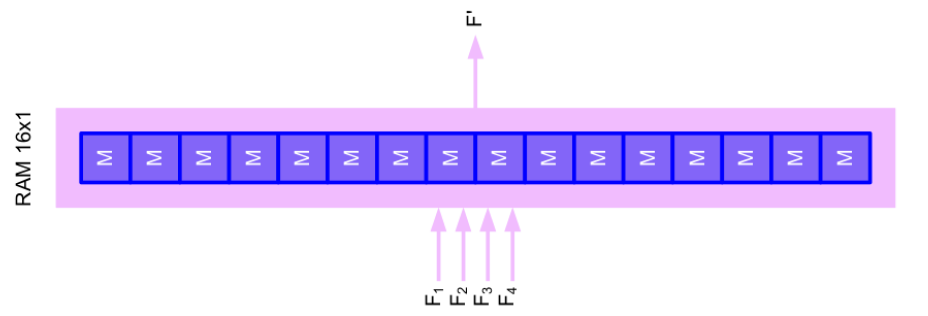
\includegraphics[width=0.4\textwidth]{./pictures/LUT.png} \\
			\textbf{Basic Logic Element (BLE) or Logic Cell:} \\
			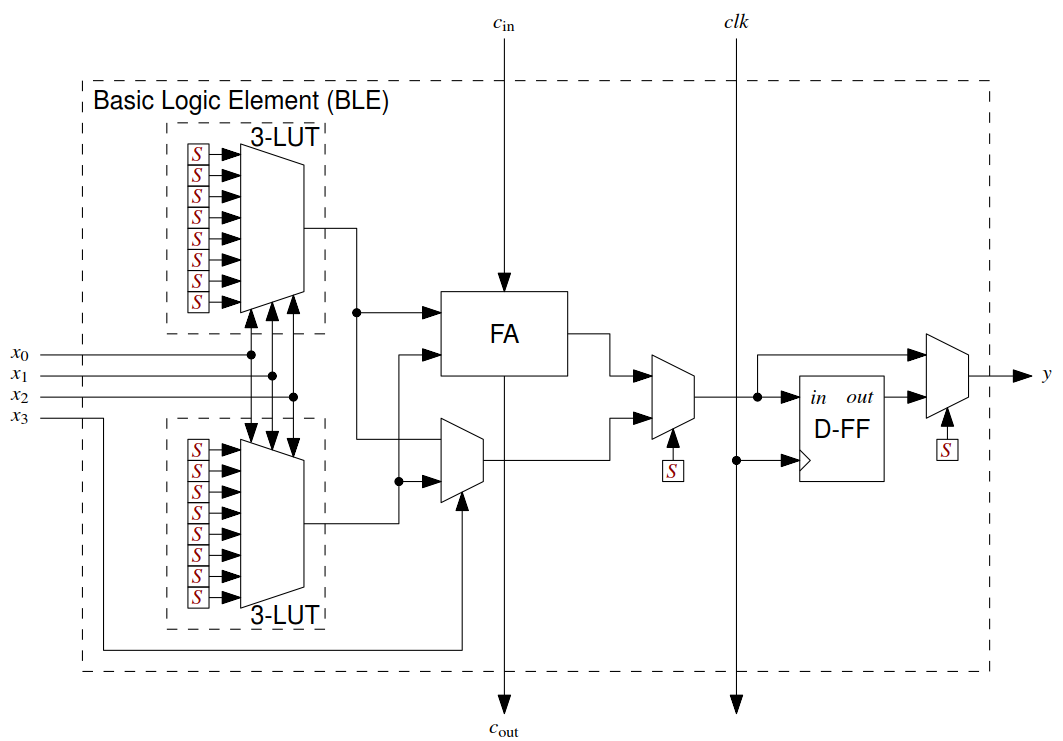
\includegraphics[width=0.4\textwidth]{./pictures/ble.png} \\
			\textbf{Switch Box (SB), Connection Box (CB):} \\
			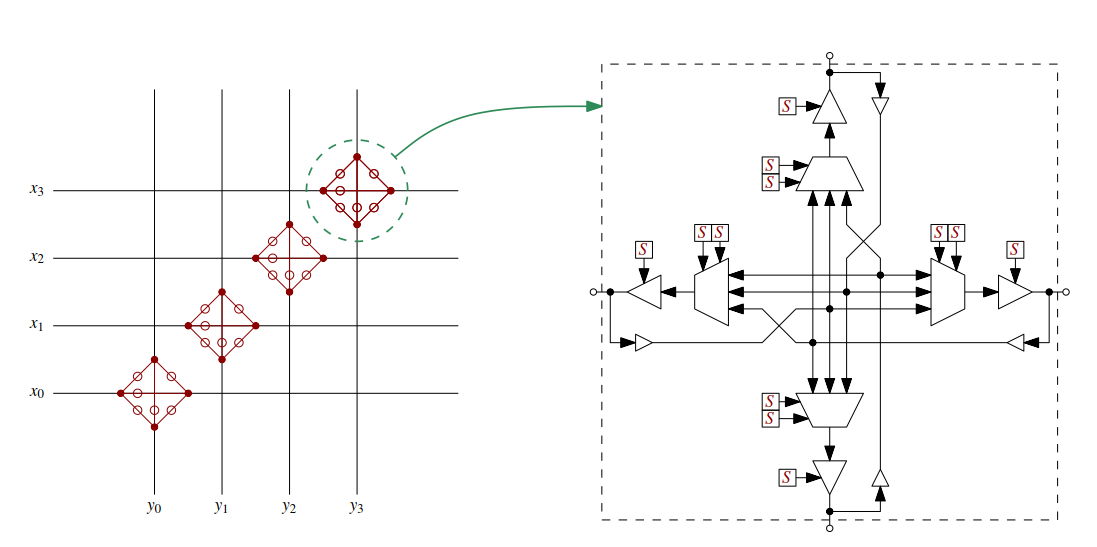
\includegraphics[width=0.4\textwidth]{./pictures/sb.png} \\
			\textbf{Configurable Logic Block (CLB):} \\
			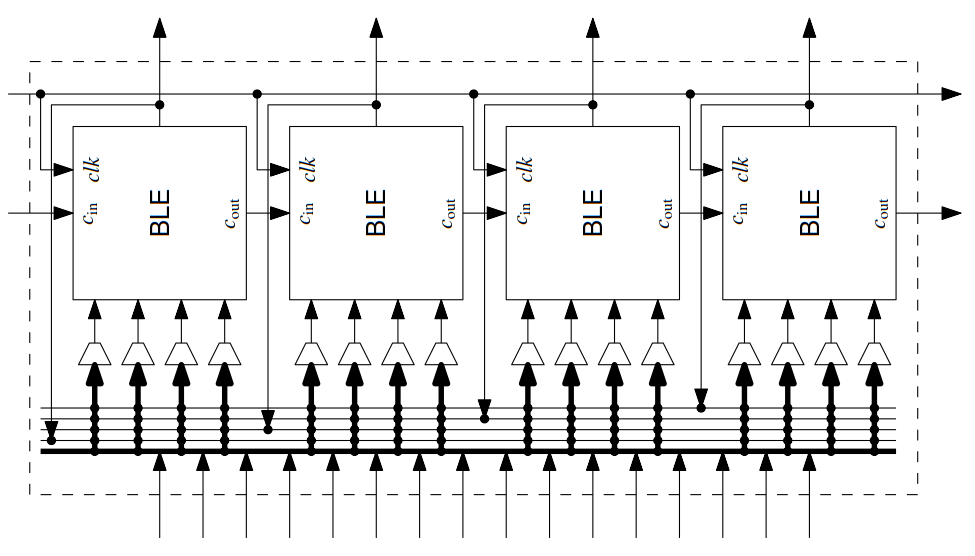
\includegraphics[width=0.4\textwidth]{./pictures/clb.png} \\ 		
			\textbf{Input/Output block (IOB):}  \\
			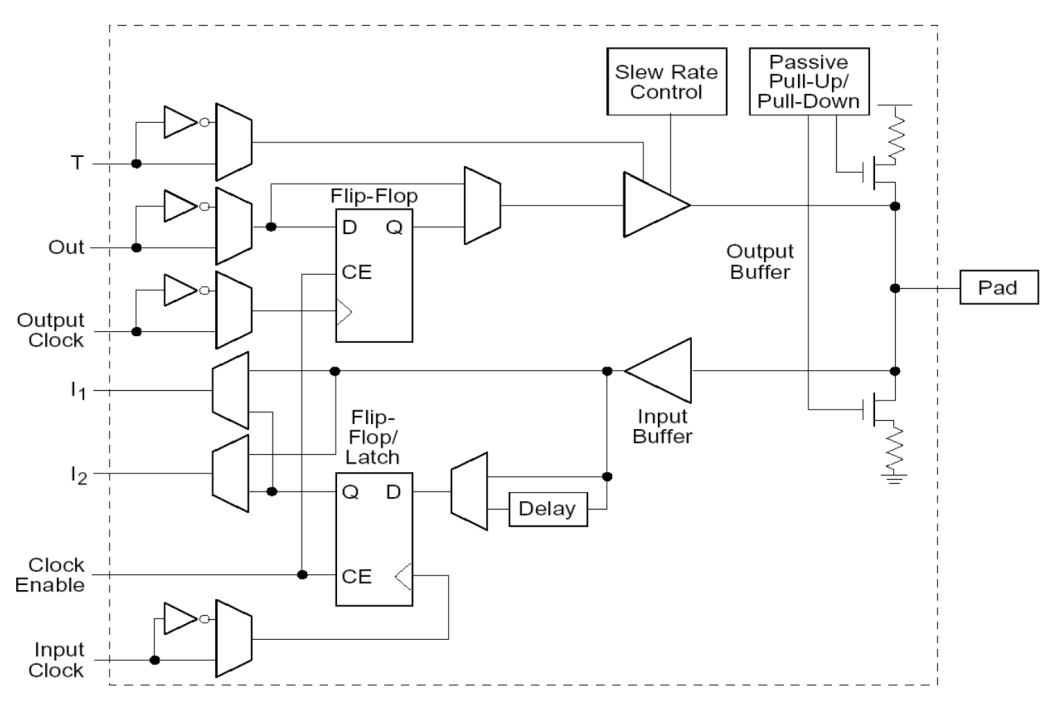
\includegraphics[width=0.4\textwidth]{./pictures/iob.png} \\
			\textbf{Dedicated Blocks (DBs):} \\
			Configurable specialized blocks implementing commonly needed functionality efficiently
			\begin{compactitem}
				\item Block SRAM
				\item Digital Clock Manager (DCM), DLL, PLL
				\item Multiplier
				\item DSP block
				\item Complete CPU cores
			\end{compactitem}
		\end{multicols}
		
	
\section{Avalon Interface}
	The Avalon interface allows you to interconnect components in Intel FPGAs using Qsys via the Avalon Bus.
	
	\subsection{Interface Types \avIntSp{4}}
		A single component can have any number of Avalon Interfaces, and also multiple instances of the same interface type. The available interface types are:
			\begin{longtable}{|>{\bfseries}p{0.3\linewidth}|p{0.65\linewidth}|}
				\hline
				Streaming Interface
					& Supports the unidirectional flow of data.\\
				\hline
				Memory Mapped Interface
					& Supports address-based read/write behaviour for master-slave connections.\\
				\hline
				Conduit Interface
					& Supports individual signals or signal groups that do not finto any other Avalon type.
					These signals can be interconnected inside a Qsys system or exported to other modules or FPGA pins.\\
				\hline
				Tri-State Conduit Interface
					& Supports off-chip peripherals. Multiple peripherals can share pins through signal multiplexing.\\
				\hline
				Interrupt Interface
					& Supports interrupts in order to signal events to other components.\\
				\hline
				Clock Interface
					& Drives or receives clocks.\\
				\hline
				Reset Interface
					& drives or receives resets.\\
				\hline	
			\end{longtable}
		
	\subsection{Avalon Memory Mapped Interface \avIntSp{13}}
		Memory mapped interfaces are components that are mapped into the global memory space. Typically the necessary amount of memory equals the space required by the component's registers. The system allocates the amount of memory to the component as can be addressed by the width of the address bus input. If the component is a memory mapped memory, the address directly represents the address location of the data (not a register).
			
		\subsubsection{Avalon MM Signals \avIntSp{15-19} \weekPageMaehne{3}{8}}
			%Some remarks to Avalon MM Signals. For a complete listing see \avIntSp{15-19}.
			\begin{longtable}{|p{0.12\linewidth}||p{0.22\linewidth}|p{0.56\linewidth}|}					
				\hline
				\textbf{Signal}
					& \textbf{Description}
					& \textbf{Remarks}\\
				\hhline{|=#=|=|}
				\texttt{address}
					& The address which is read or written to. 
					&   \textbf{Master:} The global address space unique address needs to be set.
					
					  	\textbf{Slave:} Only the component internally unique address (last few bits) are visible at the slave address input.\\
				\hline
				\texttt{write}
					& Signals a write transfer.
					& At the rising edge all signals necessary for the transfer are asserted.\\
				\hline
				\texttt{writeData}
					& Data to write.
					& Data is set for one cycle.\\
				\hline
				\texttt{read}
					& Signals a read transfer.
					& At the rising edge all signals necessary for the transfer are asserted.\\
				\hline
				\texttt{readData}
					& Data being read.
					& Data is set for one cycle.\\
				\hline
				\texttt{waitRequest}
					& Signals that transfer can not be responded to yet.
					& Asserted by the slave when it is unable to respond to a \texttt{read} or \texttt{write} request. Forces the master to wait until slave is ready. Master must not change output to the slave until \texttt{waitRequest} is deasserted.\\
				\hline
				\texttt{readDataValid}
					& When asserted, \texttt{readData} contains valid data.
					& Must be asserted for $n$ clock cycles (not necessarily consecutively) for each of the $n$ \texttt{readData} terms of a burst transfer.\\
				\hline
			\end{longtable}
		
		\subsubsection{Read and Write Transfers with fixed cycle-delay \avIntSp{27} \weekPageMaehne{3}{10}}
		\begin{multicols}{2}
			\begin{compactenum}
				\item \texttt{address}, \texttt{byteenable} and \texttt{read} are asserted after the rising edge of \texttt{clk}.
				\item The next rising edge of \texttt{clk} mrarks the end of the first and only wait-state-cycle. The \texttt{readWaitTime} is 1.
				\item The Slave asserts \texttt{readData} and \texttt{response}.
				\item \texttt{readData} and \texttt{response} are read by the master, completing the transfer.
				
				\item \texttt{address}, \texttt{byteenable} and \texttt{write} are asserted after the rising edge of \texttt{clk}.
				\item Slave reads \texttt{writeData}. The write transfer ends after 2 wait-state cycles.
			\end{compactenum}
			\begin{tikztimingtable}
				\texttt{clk} 			& LHLHLHLHLHLHL \\
				\texttt{address} 		& UDDDDUUDDDDUU \\
				\texttt{byteenable} 	& UDDDDUUDDDDUU \\
				\texttt{read} 			& LHHHHLLLLLLLL \\
				\texttt{write} 			& LLLLLLLHHHHLL \\
				\texttt{readData}		& UUUDDUUUUUUUU \\
				\texttt{response}		& UUUDDUUUUUUUU \\
				\texttt{writeData}		& UUUUUUUDDDDUU \\
				\extracode
				% Add vertical lines in two colors
				\begin{pgfonlayer}{background}
					% Add background grid lines
					\begin{scope}[gray,semitransparent,semithick,dotted]
						\vertlines{1,3,5,7,9,11,13}
					\end{scope}
				\end{pgfonlayer}
			\end{tikztimingtable} \\
		\end{multicols}
			
		\subsubsection{Read and Write Transfers with \texttt{waitRequest} \avIntSp{23} \weekPageMaehne{3}{11}}	
			\begin{multicols}{2}
				\begin{compactenum}
					\item \texttt{address}, \texttt{byteenable} and \texttt{read} are asserted after the rising edge of \texttt{clk}.
					\item Slave asserts \texttt{waitRequest}.
					\item Master waits.
					\item Slave deasserts \texttt{waitRequest} after the rising edge of clk. \texttt{readData} and \texttt{response} are set by the slave at the same time.
					\item \texttt{readData} and \texttt{response} are read by the master, completing the transfer.
					  
					\item \texttt{address}, \texttt{byteenable} and \texttt{write} are asserted after the rising edge of \texttt{clk}.
					\item Slave asserts \texttt{waitRequest}.
					\item Master waits.
					\item Slave deasserts \texttt{waitRequest} after the rising edge of clk.
					\item Slave reads \texttt{writeData}. \texttt{writeData} is valid until the next rising edge of \texttt{clk} after \texttt{waitRequest} is deasserted.
				\end{compactenum}
				\begin{tikztimingtable}
					\texttt{clk} 			& LHLMLHLHLMLHLMLHLHLHL \\
					\texttt{address} 		& UDDMDDDUUUUMUDDMDDDUU \\
					\texttt{byteenable} 	& UDDMDDDUUUUMUDDMDDDUU \\
					\texttt{read} 			& LHHMHHHLLLLMLLLMLLLLL \\
					\texttt{write} 			& LLLMLLLLLLLMLHHMHHHLL \\
					\texttt{waitRequest}	& LHHMHLLLLLLMLHHMHLLLL \\
					\texttt{readData}		& UUUMUUUDDUUMUUUMUUUUU \\
					\texttt{response}		& UUUMUUUDDUUMUUUMUUUUU \\
					\texttt{readDataValid}	& LLLMLLLHHLLMLLLMLLLLL \\
					\texttt{writeData}		& UUUMUUUUUUUMUDDMDDDUU \\
					\extracode
					% Add vertical lines in two colors
					\begin{pgfonlayer}{background}
						% Add background grid lines
						\begin{scope}[gray,semitransparent,semithick,dotted]
							\vertlines{1,3,5,7,9,11,13,15,17,19}
						\end{scope}
					\end{pgfonlayer}
				\end{tikztimingtable}	\\ \\ \\
			\end{multicols}		
	
		\subsubsection{Burst Write Transfer with \texttt{waitRequest} \avIntSp{32} \weekPageMaehne{4}{4}}	
			\begin{multicols}{2}
				\begin{compactenum}
					\item The master asserts \texttt{address}, \texttt{burstcount}, \texttt{write}, and drives the first unit of \texttt{writedata}.
					\item The slave asserts \texttt{waitrequest}.
					\item Master waits.
					\item \texttt{waitrequest} is low. The slave captures \texttt{addr1}, \texttt{burstcount}, and the first unit of \texttt{writedata}. On subsequent cycles of the transfer, \texttt{address} and \texttt{burstcount} are ignored.
					\item The slave captures the second unit of \texttt{data} at the rising edge of \texttt{clk}.
					\item The burst is paused while \texttt{write} is deasserted.
					\item The slave captures the third unit of \texttt{data} at the rising edge of \texttt{clk}.
					\item The slave asserts \texttt{waitrequest}.
					\item Master waits.
					\item The slave captures the last unit of \texttt{data} on this rising edge of \texttt{clk}.
				\end{compactenum}
				\begin{tikztimingtable}
					\texttt{clk} 				& LHLHLHLHLMLHLHLHLHL \\
					\texttt{address} 			& U4D{addr1}UUUUMUUUUUUUUU \\
					\texttt{begimbursttransfer} & LHHLLLLLLMLLLLLLLLL \\
					\texttt{burstcount} 		& U4D{4}UUUUMUUUUUUUUU \\
					\texttt{write} 				& LHHHHHHLLMLHHHHHHLL \\
					\texttt{writeData}			& U4D{d1}2D{d2}UUMU2D{d3}4D{d4}UU \\
					\texttt{waitRequest}		& LHHLLLLLLMLLLHHLLLL \\					
					\extracode
					% Add vertical lines in two colors
					\begin{pgfonlayer}{background}
						% Add background grid lines
						\begin{scope}[gray,semitransparent,semithick,dotted]
							\vertlines{1,3,5,7,9,11,13,15,17,19}
						\end{scope}
					\end{pgfonlayer}
				\end{tikztimingtable}	\\ \\ \\ \\ \\ \\
			\end{multicols}		
		
		\subsubsection{Avalon MM Slave \weekMaehne{3}}
			The \texttt{simplePIO}-IP allows to interface external elements such as LEDs, buttons, switches. It has the following functionality:
			\begin{compactitem}
				\item Each pin can be set as input or output. The direction can be read back.
				\item The direction is set by \texttt{RegDir}; (0 : input / 1 : output)
				\item The state of the port can be read in at pin level by \texttt{RegPin}
				\item The state value is stored in the register \texttt{RegPort}
			\end{compactitem} \ \\
		
			The register map of this IP block looks as follows: \\
			\begin{tabular}{|p{0.1\textwidth}|p{0.1\textwidth}|p{0.1\textwidth}|}
				\hline
				\textbf{Addr} & \textbf{Write} & \textbf{Read} \\
				\hline
				0x0 & \texttt{RegDir} & \texttt{RegDir} \\ \hline
				0x1 & - & \texttt{RegPin} \\ \hline
				0x2 & \texttt{RegPort} & \texttt{RegPort} \\ \hline
				0x3 & \texttt{RegSet} & - \\ \hline
				0x4 & \texttt{RegClr} & - \\ \hline
			\end{tabular}
			\begin{multicols}{2}		
				\lstinputlisting[style=VHDL]{./src/simplePIO.vhdl}
			\end{multicols}			
			
%		\subsubsection{Avalon MM Master}
%			\todo{Sinnvoll dieses Kapitel?, weiss nicht ob das benötigt wird}		
		
\section{Cache \weekDoran{3}}
	The cache is completely transparent to the user. It can not explicitly be filled (e.g. using a DMA). The only way to fill the cache is by executing code or data (except for dirty tricks).
	
	The cache is used to store often executed code or data in a closely located storage.
	
	\subsection{Cache Types}
		\begin{table}[H]
			\centering
			\begin{tabular}{|p{0.3\linewidth}|p{0.65\linewidth}|}
				\hline
				Level 1 Cache
					& Cache that is located closest to the processor. Usually on-chip memory. Also called first level, primary or L1 cache.\\
				\hline
				Level 2 Cache
					& Located downstream of L1 Cache and usually off-chip memory. Also called second level, secondary or L2 cache.\\
				\hline
				Level 3 Cache
					& Located downstream of L2 Cache and usually off-chip memory. Also called third level, tertiary or L3 cache.\\
				\hline	
			\end{tabular}
			\caption{Cache Types}
		\end{table}
		
	\subsection{Cache Behaviour \weekPageDoran{3}{9}}
	
		\begin{table}[H]
			\centering
			\begin{tabular}{|p{0.3\linewidth}|p{0.65\linewidth}|}
				\hline
				\multicolumn{2}{|c|}{Controller is looking for a memory item}\\
				\hline
				\textbf{Cache hit}
					& Memory item is found in cache. Controller can be served faster than without cache due to the its proximity to the controller.\\
				\hline
				\textbf{Cache miss}
					& Memory item is not found in cache. Controller is served slower than without Cache due to the checking of the cache before looking in the memory. The \textbf{cache directory} will decide whether a copy of the required datum is in the memory and the \textbf{cache controller} will manage the interaction with system memory, formulated by \textbf{cache policies}. When loading data, it will also be loaded into the cache.\\
				\hline
			\end{tabular}
			\caption{Cache Behaviour}
		\end{table}
		
	\subsection{Cache Structure \weekPageDoran{3}{9}}
		\subsubsection{Cache Addressing in Direct Mapped Cache}
			\begin{table}[H]
				\centering
				\begin{tabular}{|p{0.2\linewidth}|p{0.75\linewidth}|}
					\hline
					\textbf{Line number}
						& Represents the lowest significant bits of the main memory address. It is unique over the whole cache and thus the size depends on the cache. Therefore only one datum of each with the same address in the main memory can be represented in the cache.\\
					\hline
					\textbf{Address Tag}
						& Represents the most significant bits of the main memory address (Complete address without cache line number).\\
					\hline
				\end{tabular}
				\caption{Cache Addressing in Direct Mapped Cache}
			\end{table} 
			
		\subsubsection {1 Word}
		
			\begin{table}[H]
				\centering
				\begin{tabular}{p{0.15\linewidth}|p{0.06\linewidth}|p{0.06\linewidth}|p{0.06\linewidth}|p{0.2\linewidth}|p{0.2\linewidth}|}
					\cline{2-6}
						\textbf{Line number}
							& \textbf{Valid}
							& \textbf{Dirty}
							& \textbf{Locked}
							& \textbf{Address tag}
							& \textbf{Data}\\
					\cline{2-6}
						0x00
							& 1
							& 1
							& 0
							& Address tag 0
							& Valid data\\
					\cline{2-6}
						0x01
							& 0
							& 1
							& 0
							& N/A
							& Garbage\\
					\cline{2-6}
				\end{tabular}
				\caption{1 Word cache structure}
			\end{table}	
			
		\subsubsection {2 Word}
		
			\begin{table}[H]
				\centering
				\begin{tabular}{p{0.15\linewidth}|p{0.06\linewidth}|p{0.06\linewidth}|p{0.06\linewidth}|p{0.2\linewidth}|p{0.2\linewidth}|}
					\cline{2-6}
						\textbf{Line number}
							& \textbf{Valid}
							& \textbf{Dirty}
							& \textbf{Locked}
							& \textbf{Address tag}
							& \textbf{Data}\\
					\cline{2-6}
						0x00
							& 1
							& 1
							& 0
							& Address tag 0
							& Valid data\\
					\cline{2-6}
						0x01
							& 
							& 
							& 
							& 
							& Valid data\\
					\cline{2-6}
						0x02
							& 0
							& 1
							& 0
							& N/A
							& Garbage\\
					\cline{2-6}
						0x03
							& 
							& 
							& 
							& 
							& Garbage\\
					\cline{2-6}
				\end{tabular}
				\caption{2 Word cache structure}
			\end{table}	

	\subsection{Cache Policies}
		\subsubsection{General}
			A \textbf{line fill/update} is when a cache line is updated with a new datum. A \textbf{compulsory line fill/update} is such an update that could not have been avoided using a better cache policy.
			
		\subsubsection{Reading from Cache}
			\begin{table}[H]
				\centering
				\begin{tabular}{|p{0.3\linewidth}|p{0.65\linewidth}|}
					\hline
					\textbf{Look-aside implementation}
						& All signals are access main memory, regardless of hit or miss.\\
					\hline
					\textbf{Look-through / in-line implementation}
						& Cache controller decides whether to initiate system memory read/write. Massively reduces CPU-required bandwidth at the cost of \textbf{lookup penalty} (time required to decide that system memory access is required). \\
					\hline
				\end{tabular}
				\caption{Cache Read Policies}
			\end{table}
			
		\subsubsection{Writing to Cache}
			\begin{table}[H]
				\centering
				\begin{tabular}{|p{0.3\linewidth}|p{0.65\linewidth}|}
					\hline
					\textbf{Write-through policy}
						& Both the cache and system memory are updated in order to avoid cache coherence problems.\\
					\hline
					\textbf{Copy-back policy}
						& Only the cache data is updated. This causes cache coherence problems. Simplest method is to set a dirty bit in the cache. When a cache line is replaced the system memory is updated with the new value in the cache (Data is evicted).\\
					\hline
				\end{tabular}
				\caption{Cache Write Policies}
			\end{table}
			
	\subsection{Cache Locking}
		Code and data can be locked in cache.
		
		\todo{Fill this section}
		
	\subsection{Cache Aware Programming}
		\subsubsection{Software Pre-Fetching \weekPageDoran{3}{27}}
			\begin{itemize}
			  \item Some compilers offer pre-fetching and pre-fetching instruction insertion.
			  \item Manual insertion generally preferred.
			\end{itemize}
			
		\lstinputlisting[style=CPP, caption=Software Pre-Fetching]{./src/prefetch.cpp}
		
		\subsubsection{Hardware Pre-Fetching \weekPageDoran{3}{31}}
			A memory access is registered, on the second access the stride (difference between second and first address) is also registered. If the hardware thinks the stride is stable then it starts pre-fetching blocks with this stride.
			
		\subsubsection{Data Access Optimisation \weekPageDoran{3}{34-37}}		
			Minimise cache misses.
			
			\begin{table}[H]
				\centering
				\begin{tabular}{|p{0.3\linewidth}|p{0.65\linewidth}|}
					\hline
					\textbf{Loop Interchange}
						& Interchange loop indices. Instead of iterating row-wise iterate column-wise or the other way around.\\
					\hline
					\textbf{Loop Fusion}
						& Combine multiple loops into one. \\
					\hline
					\textbf{Loop Blocking/Tiling}
						& Instead of iterating column or row wise, iterate in blocks or tiles. (This causes more loops than row or column wise)\\
				\end{tabular}
				\caption{Loop Transformations}
			\end{table}
			
			\todo{Add source code and/or images for loop transformations.}
			
	\subsection{Cache Coherence}
		\subsubsection{Cache Snooping Protocol MSI}
			\begin{table}[H]\centering
				\begin{tabular}{|>{\bfseries}p{0.1\textwidth}|p{0.36\textwidth}|>{\bfseries}p{0.1\textwidth}|p{0.36\textwidth}|}
					\hline
					\multicolumn{2}{|l|}{\textbf{Memory block states}}
						& \multicolumn{2}{|l|}{\textbf{Cache line states}}\\
					\hline
					Clean
						& In one or more caches and up-to-date in memory.
						& Shared
						& The block is unmodified and exists in read-only state in at least one cache.\\
					\hline
					Dirty
						& In exactly one cache. (updated in cache, not in memory)
						& Invalid
						& The block is either not present in the current cache or has been invalidated. It must be fetched from memory.\\
					\hline
					Uncached
						& In no caches.
						& Modified/\newline\ Exclusive
						& The block has been modified in the cache, and not updated in the memory yet.\\
					\hline
				\end{tabular}
			\end{table}
			
			\begin{figure}[H]\centering
				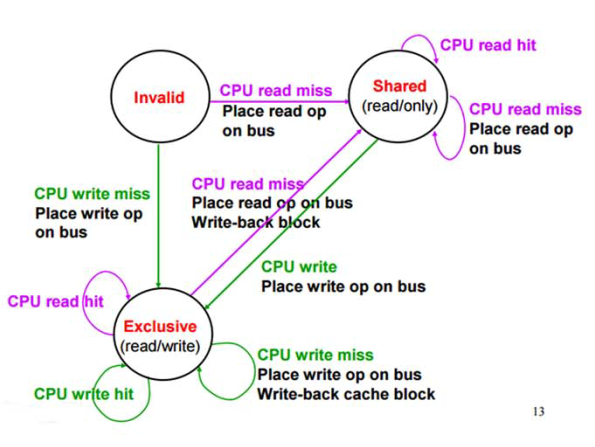
\includegraphics[scale=0.5]{./pictures/MSIProtocol.png}
				\caption{MSI Protocol cache line states}
			\end{figure}
\end{document}